% !TeX spellcheck = de_DE
\documentclass{alex_hü}

\name{Alexander Helbok}
\course{PS Astrophysics}
\hwnumber{1}


\begin{document}
\renewcommand{\labelenumi}{\alph{enumi})}


\begin{mybox}{Hydrostatic equilibirum}
	\centering \( \rho(r) = \rho_c\left( 1 - \tfrac{r}{R} \right) \)
	\tcblower
	\begin{enumerate}
		\item \(  \)
		\begin{flalign*}
			\dv{m}{r} &= 4\pi r^2\rho(r) 
				= 4\pi r^2\rho_c\left( 1 - \tfrac{r}{R} \right) &&\\
			\uint[0,m(r)]{1}{\tilde{m}} &= \uint[0,r]{4\pi \tilde{r}^2\rho_c\left( 1 - \tfrac{\tilde{r}}{R} \right)}{\tilde{r}} &&\\
			m(r) &= \dl{4\pi\rho_c \left( \tfrac{r^3}{3} - \tfrac{r^4}{4R} \right)} &&
		\end{flalign*}
	\tcbline
		\item \(  \)
		\begin{flalign*}
			\dv{P}{r} &= -G\tfrac{m(r)\rho(r)}{r^2} 
				= -G\pi\rho_c^2 \left( -\tfrac{4r}{3} + \tfrac{7r^2}{3R} - \tfrac{r^3}{R^2} \right) &&\\
			\uint[Pc,P]{1}{\tilde{P}} &= \uint[0,r]{-G\tfrac{m(\tilde{r})\rho(\tilde{r})}{\tilde{r}^2}}{\tilde{r}} &&\\
			P(r) &= -G\pi\rho_c^2 \left( -\tfrac{2r^2}{3} + \tfrac{7r^3}{9R} - \tfrac{r^4}{4R^2} \right) - P_c &&\\
			P(R) &= 0 \quad\Rightarrow\quad P_c = -G\pi\rho_c^2 \left( -\tfrac{2R^2}{3} + \tfrac{7R^2}{9} - \tfrac{R^2}{4} \right)
				= G\pi\rho_c^2 \tfrac{5R^2}{36} &&\\
			\rho_c^2 &= \tfrac{36P_c}{5G\pi R^2} &&\\[4ex]
			\Rightarrow P(r) &= \dl{P_c\left(1 - \tfrac{24 r^2}{5 R^2} + \tfrac{28r^3}{5R^3} - \tfrac{9 r^4}{5 R^4} \right)} &&
		\end{flalign*}
	\tcbline
		\item \(  \)
		\begin{flalign*}
			\frac{P(x=\tfrac{r}{R})}{P_c} &= 1 - \frac{24}{5}x^2 + \frac{28}{5}x^3 - \frac{9}{5}x^4 &&
		\end{flalign*}
		\begin{minipage}{\textwidth}
			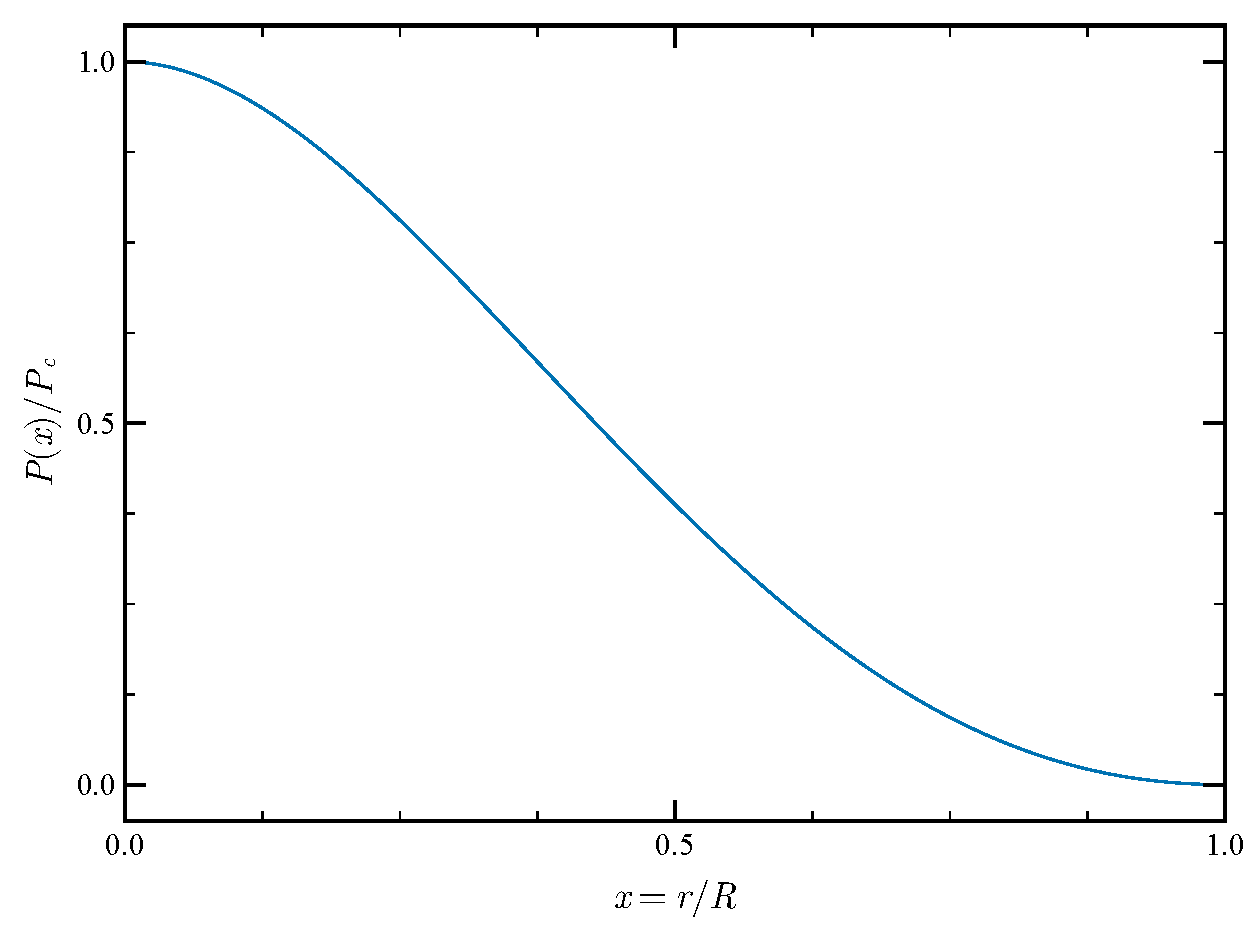
\includegraphics[width=0.85	\textwidth]{P(x)}
		\end{minipage}
	\end{enumerate}
\end{mybox}

\end{document}